\documentclass[10pt]{beamer}

\usetheme[progressbar=frametitle]{metropolis}
\usepackage{appendixnumberbeamer}

\usepackage{booktabs}
\usepackage[scale=2]{ccicons}
\usepackage{bbm}

\usepackage{pgfplots}
\usepgfplotslibrary{dateplot}

\usepackage{xspace}
\newcommand{\themename}{\textbf{\textsc{metropolis}}\xspace}

\title{Labor Markets and Technological Change: }
\subtitle{Evidence from Electronic Health Records}
% \date{\today}
\date{}
\author{Hanna Glenn}
\institute{Emory University}
% \titlegraphic{\hfill\includegraphics[height=1.5cm]{logo.pdf}}

\begin{document}

\setbeamercolor{background canvas}{bg=white}


\maketitle

\section[Motivation]{Motivation}

\begin{frame}[fragile]{Big Picture}
How does technology impact employment?
                \vspace{2mm}
    \begin{itemize}
        \item Displacement?
                \vspace{2mm}
        \item Productivity?
    \end{itemize}
                \vspace{4mm}
Investigated in different ways
                \vspace{2mm}
    \begin{itemize}
        \item Computerization and white collar jobs
                \vspace{2mm}
        \item Machinery and factory workers
    \end{itemize}
                \vspace{4mm}
                \pause
\begin{alertblock}{$\rightarrow$ This paper considers this question in the context of healthcare and physician labor markets}\end{alertblock}
\end{frame}


\begin{frame}[fragile]{What is an Electronic Health Record (EHR)?}
Health information stored digitally in a software
                \vspace{4mm}
\begin{center}
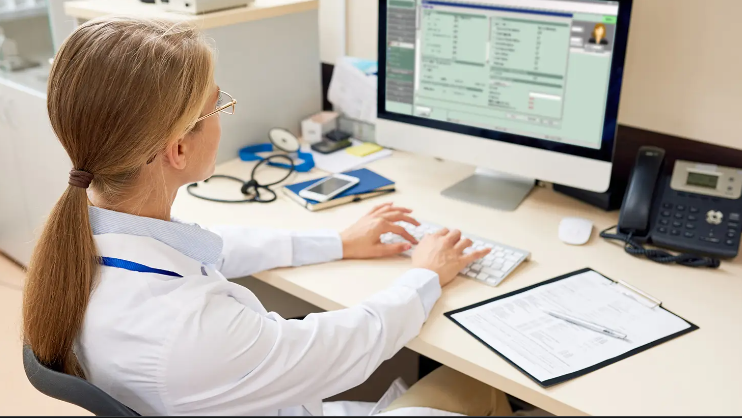
\includegraphics[scale=.4]{Objects/EHR_picture.PNG}
\end{center}
\end{frame}



\begin{frame}{Adoption in Hospitals}
\centering
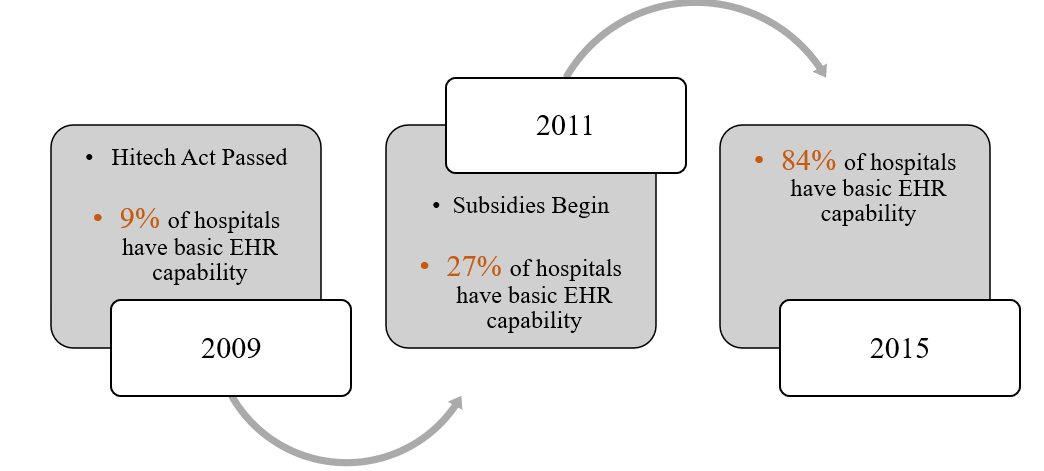
\includegraphics[scale=.4]{graphics/timeline.PNG}
\end{frame}



\begin{frame}{Physician Response to EHRs}
\centering

\includegraphics[scale=.3]{graphics/News Clip3.PNG}

                \vspace{4mm}
                

\includegraphics[scale=.3]{graphics/News Clip2.PNG}
\end{frame}



\begin{frame}{This Paper}
Did EHR implementation in hospitals affect physician labor market decisions?
                \vspace{4mm}
\begin{center}
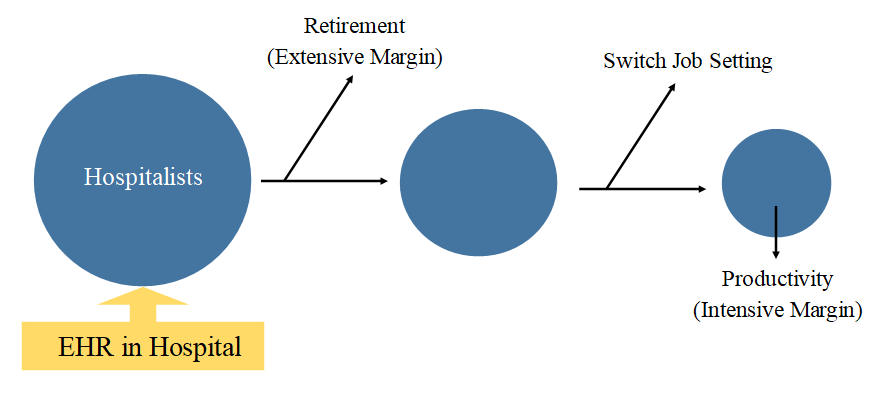
\includegraphics[scale=.4]{Objects/EHR_FlowChart_General.PNG}
\end{center}
\end{frame}



\section{Data and Analysis}

\begin{frame}[fragile]{Data}
Panel of hospitalists from 2009-2017 with information on whether the hospital uses an EHR and various labor market outcomes\\
                \vspace{3mm}
\begin{itemize}
    \item EHR information ends in 2015, so I limit to only those who were exposed by 2015
\end{itemize}
\end{frame}


\begin{frame}{Difference in Difference Analysis}
Treatment: Exposure to EHR\\
                \vspace{4mm}
Since I have staggered treatment timing, I use Callaway and Sant'Anna (2021) average group time treatment effects:
$$ATT(g,t)=\mathbbm{E}[Y_t(g)-Y_t(0)|G_g=1]$$
                \vspace{3mm}
\begin{itemize}
    \item Not-yet-treated units
    \item Aggregate to get familiar event study plot
\end{itemize}
\end{frame}


\begin{frame}{Data}
\centering
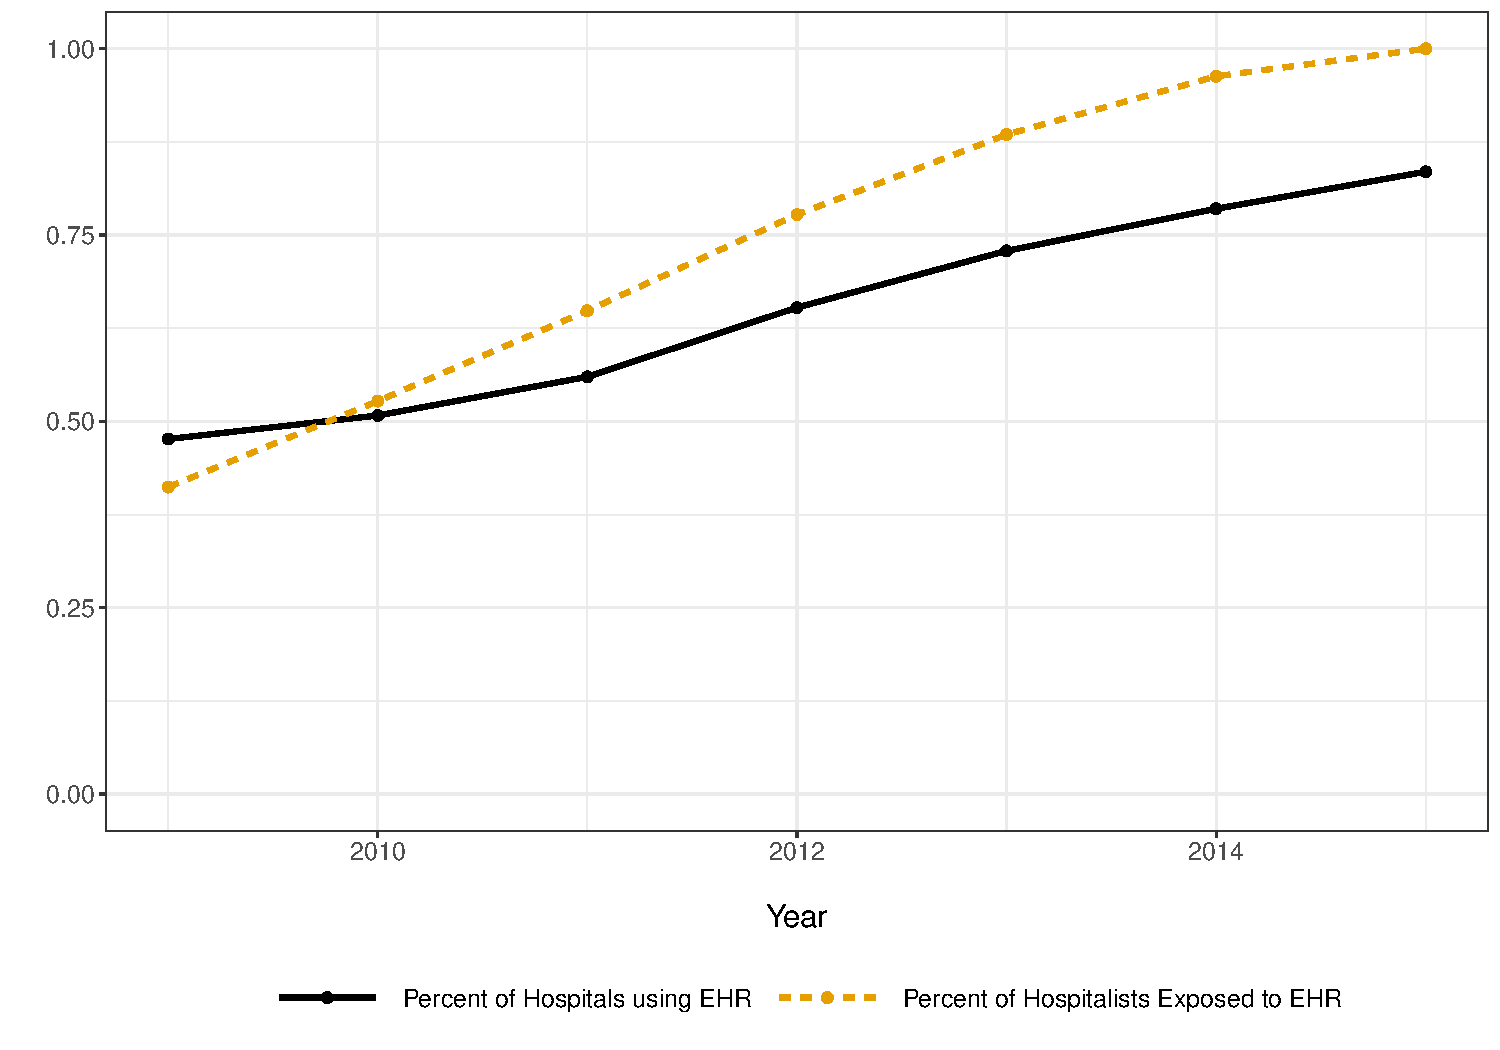
\includegraphics[scale=.4]{Objects/sum_stats_year.pdf}
\end{frame}


\begin{frame}{Assumptions}
\begin{enumerate}
    \item No reversal of treatment
                \vspace{3mm}
    \item No anticipation of treatment (can be relaxed)
                \vspace{3mm}
    \item Parallel trends
\end{enumerate} 
\end{frame}


\section{Retirement}


\begin{frame}{Retirement}
\centering
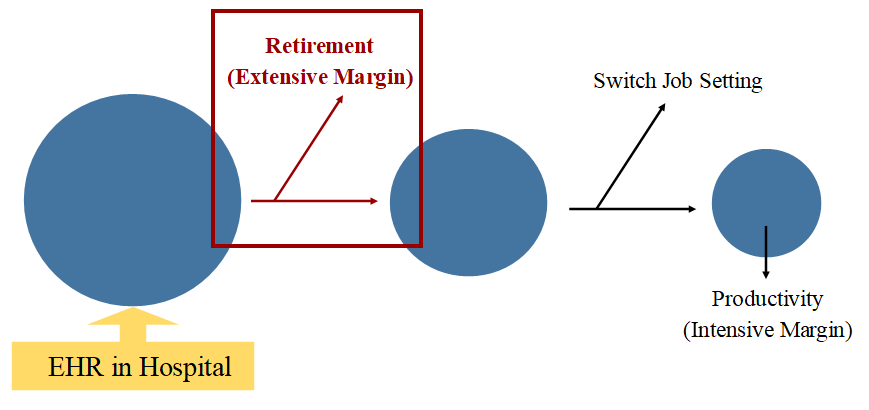
\includegraphics[scale=.4]{Objects/EHR_FlowChart_Retire.PNG}
\end{frame}


\begin{frame}{Retirement Variable}
Indicator equal to 1 if physician drops out of the data\\
                    \vspace{3mm}
\begin{itemize}
    \item No longer sees patients
\end{itemize}
\end{frame}

\begin{frame}{Physician Incentives}
Decision to retire is different than we usually think
                \vspace{3mm}
\begin{itemize}
    \item Retirement is thought of as a function of pensions, and sometimes depends on shocks such as health or job loss\\ \scriptsize{(Hall and Johnson 1980, ILRR), (Gordon and Blinder 1980, J Public Econ), (Hamermesh 1985, JOLE)}
                \vspace{3mm}
                \normalsize
    \item On average, physicians plan to retire at age 60 but don't actually retire until age 69 \scriptsize{(Collier 2017)}
\end{itemize}
\end{frame}

\begin{frame}{Physician Incentives}
Unique set of incentives for which a shock to the work setting \textit{may} lead to retirement more-so than other occupations, for which studies yield mixed results\\
\scriptsize{(Schleife 2006, Labour; Cavapozzi et al 2013, AE; Roger et al 2006, EJ; Friedburg 2003, ILRR)}\\
                \vspace{15mm}
                \normalsize
Related studies find that well educated workers exited at higher rates due to computerization\\
\scriptsize (Willis and Hudomiet 2021, Labour), (Dillender and Forsythe 2022, NBER)
\end{frame}

\begin{frame}{Leaving Clinical Setting}
Retirement is defined using whether the physician sees patients
                \vspace{3mm}
\begin{itemize}
    \item Physicians of any age could choose to leave a clinical setting
\end{itemize}
\end{frame}
\begin{frame}{Retirement}
\begin{figure}[ht]
    \centering
    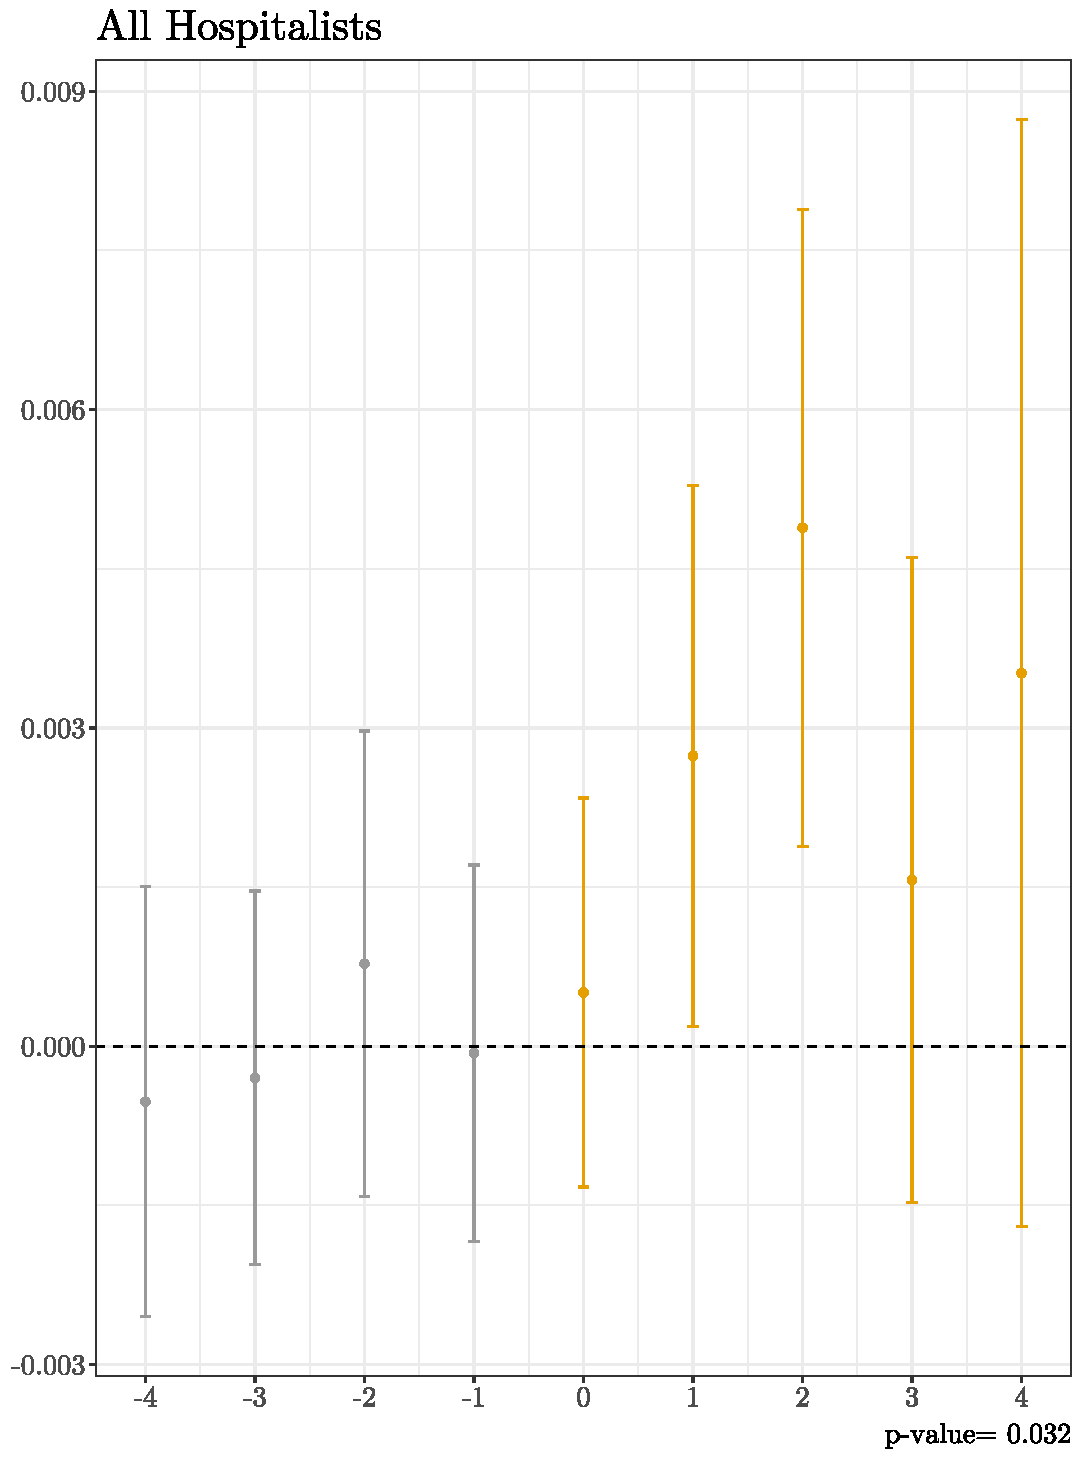
\includegraphics[scale=.35]{Objects/Presentation_retire_all.pdf}
\end{figure}
$\rightarrow$ EHR exposure led to a .003 (.0045) percentage point increase in the likelihood of retirement in the first (second) year after exposure (10\% and 15\% increase relative to the mean)
\end{frame}

\begin{frame}{Retirement: Age Groups}
\begin{figure}[ht]
\centering
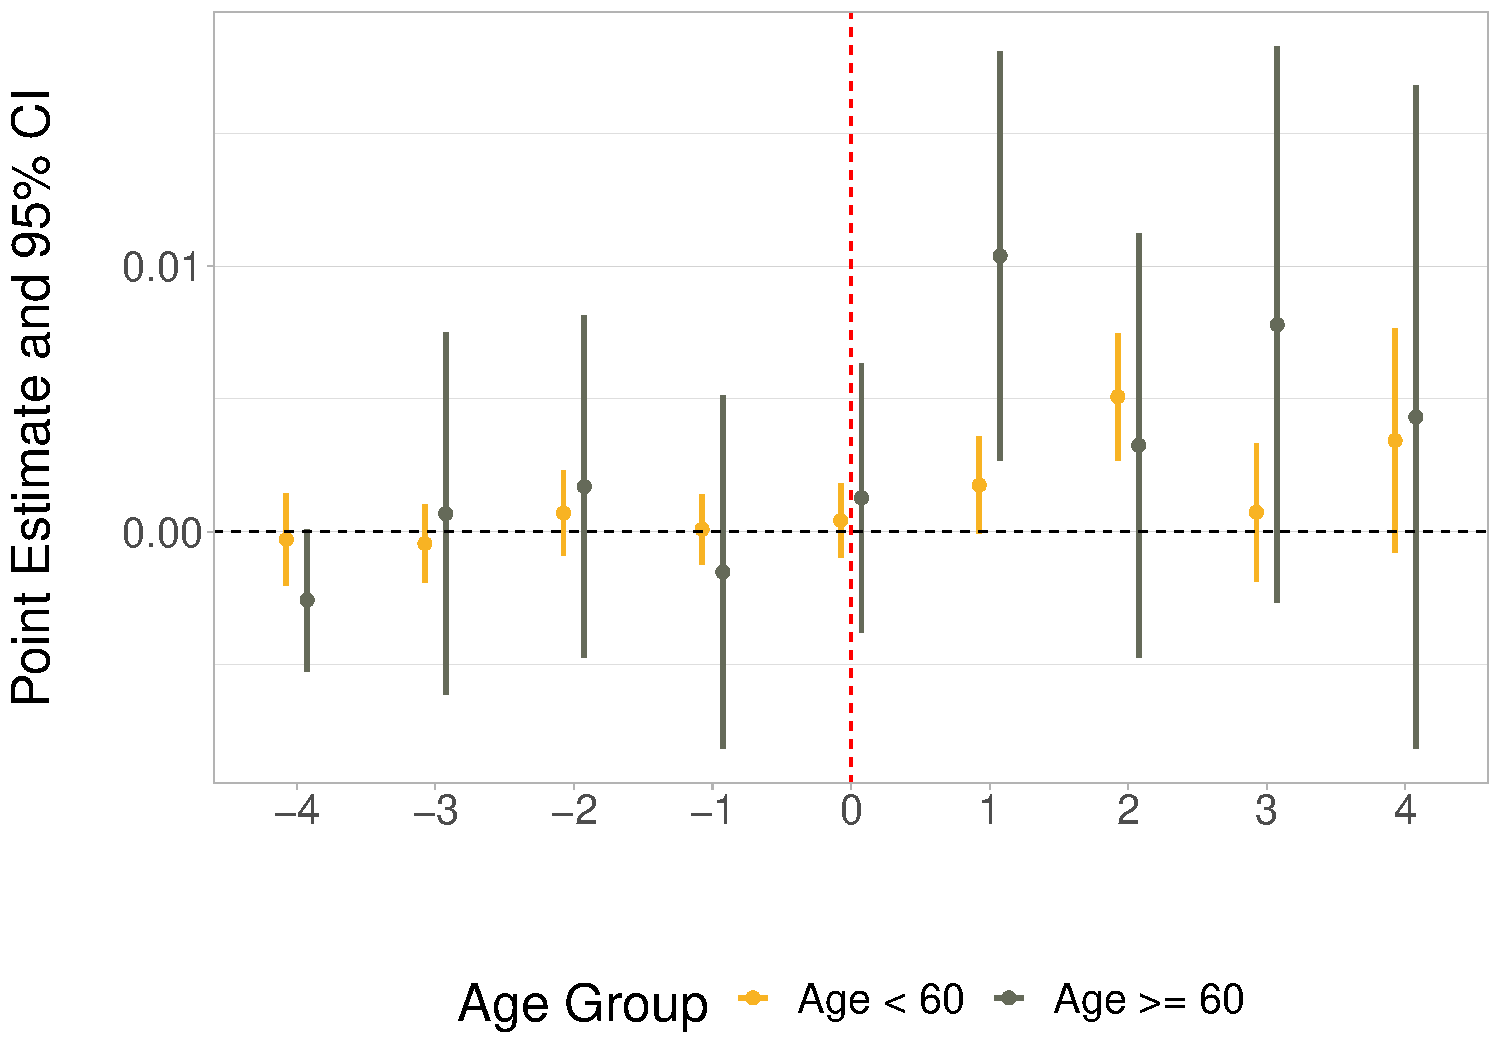
\includegraphics[scale=.35]{Objects/Presentation_retire_ages.pdf}
\end{figure}
$\rightarrow$ Older: 25\% increase relative to the mean in the first year, but 0 in the second\\
$\rightarrow$ Younger: 16\% increase in second year
\end{frame}



\section{Job Setting}




\begin{frame}{Changing Job Setting}
\centering
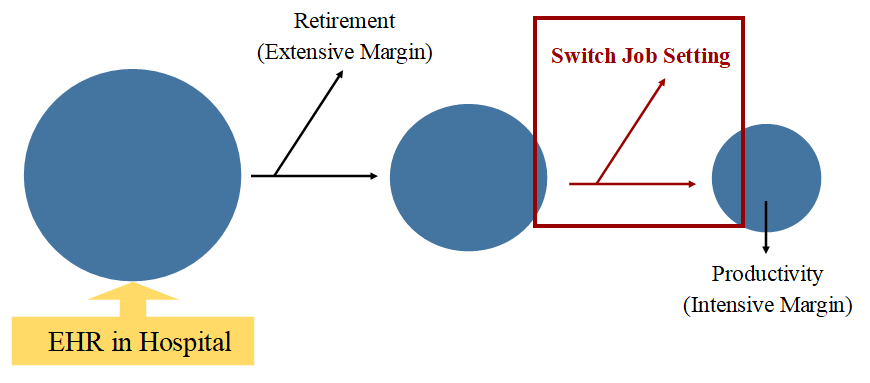
\includegraphics[scale=.5]{Objects/EHR_FlowChart_JobSwitch.PNG}
\end{frame}

\begin{frame}{Job Setting Variables}
\begin{enumerate}
    \item Indicator for working in office or not
                    \vspace{3mm}
    \item Indicator for whether the physician changed zip code
\end{enumerate}
\end{frame}



\begin{frame}{Physician Incentives}
Most physicians will not be induced to retire because of EHRs
\begin{itemize}
    \item Another way to avoid (or be exposed to) new technology is to switch location of practice
    \begin{itemize}
                \vspace{3mm}
        \item Literature shows job switching is closely tied to job satisfaction\\ \scriptsize (Aklerlof, Rose and Yellen 1988, Brookings), (Chadi and Hetschko 2017, JEMS)
    \end{itemize}
                \vspace{6mm}
                \pause
    \item The cost associated with switching depends on the strength of the tie with the hospital
    \end{itemize}
\end{frame}

\begin{frame}{Results: Indicator for Working in Office}
\begin{figure}[ht]
    \centering
    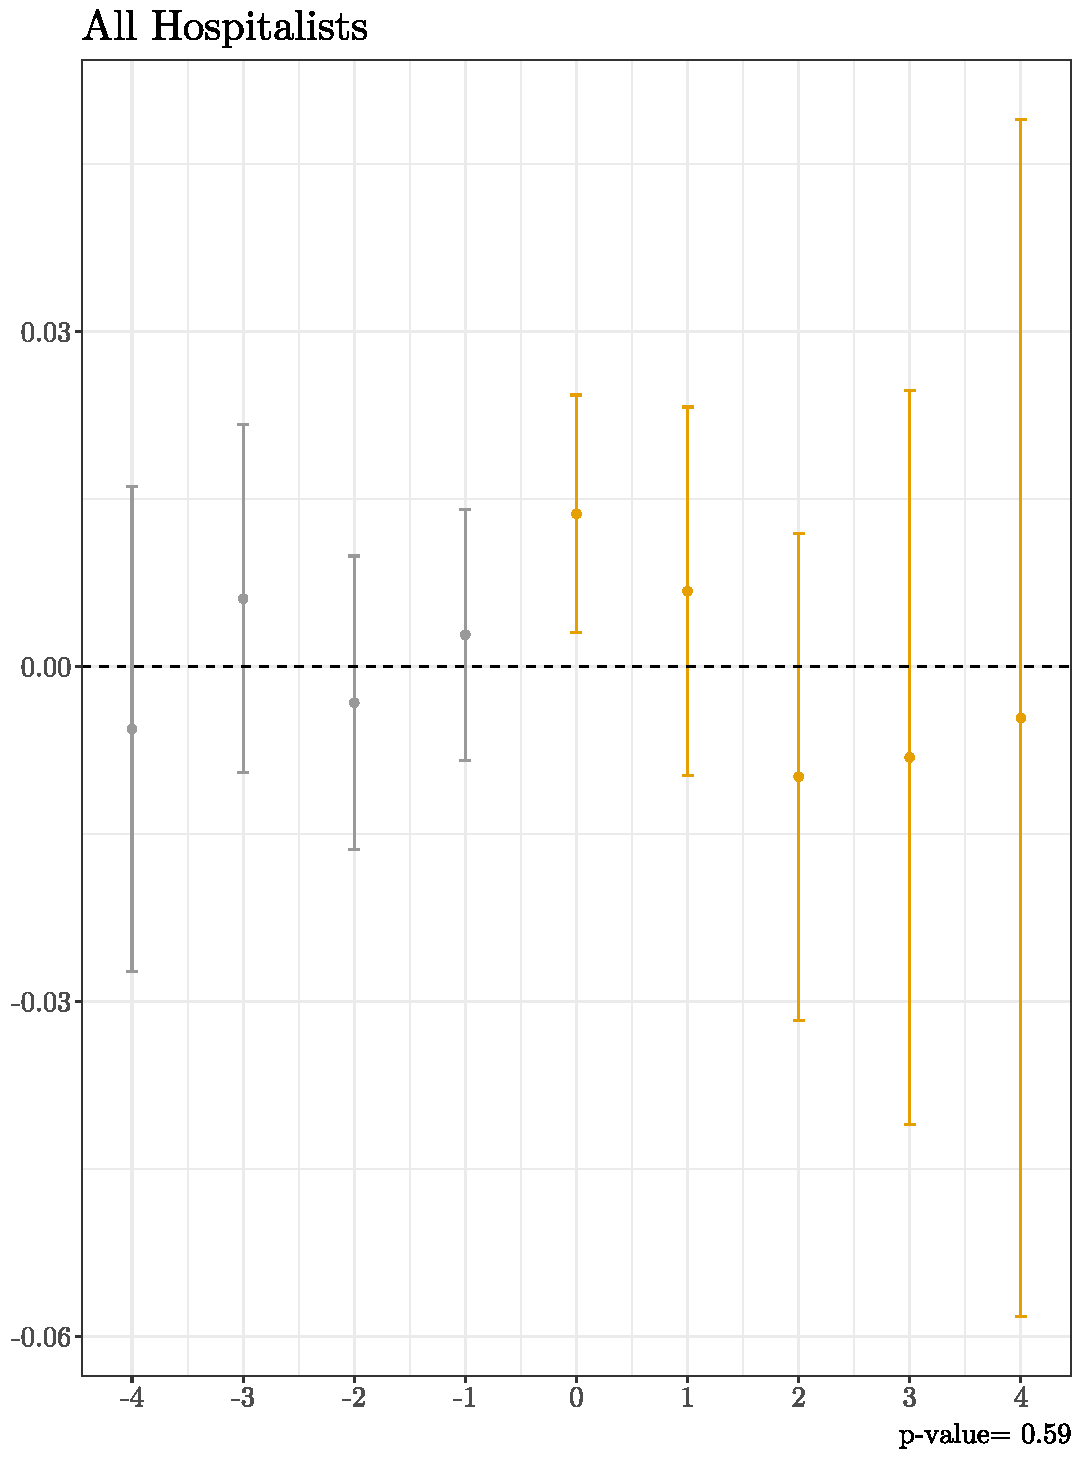
\includegraphics[scale=.35]{Objects/Presentation_office_all.pdf}
\end{figure}
$\rightarrow$ 4.6\% increase relative to the mean\\
$\rightarrow$ Driven by young physicians
\end{frame}

\begin{frame}{Results: Indicator for Changing Zip Codes}
\begin{figure}[ht]
    \centering
    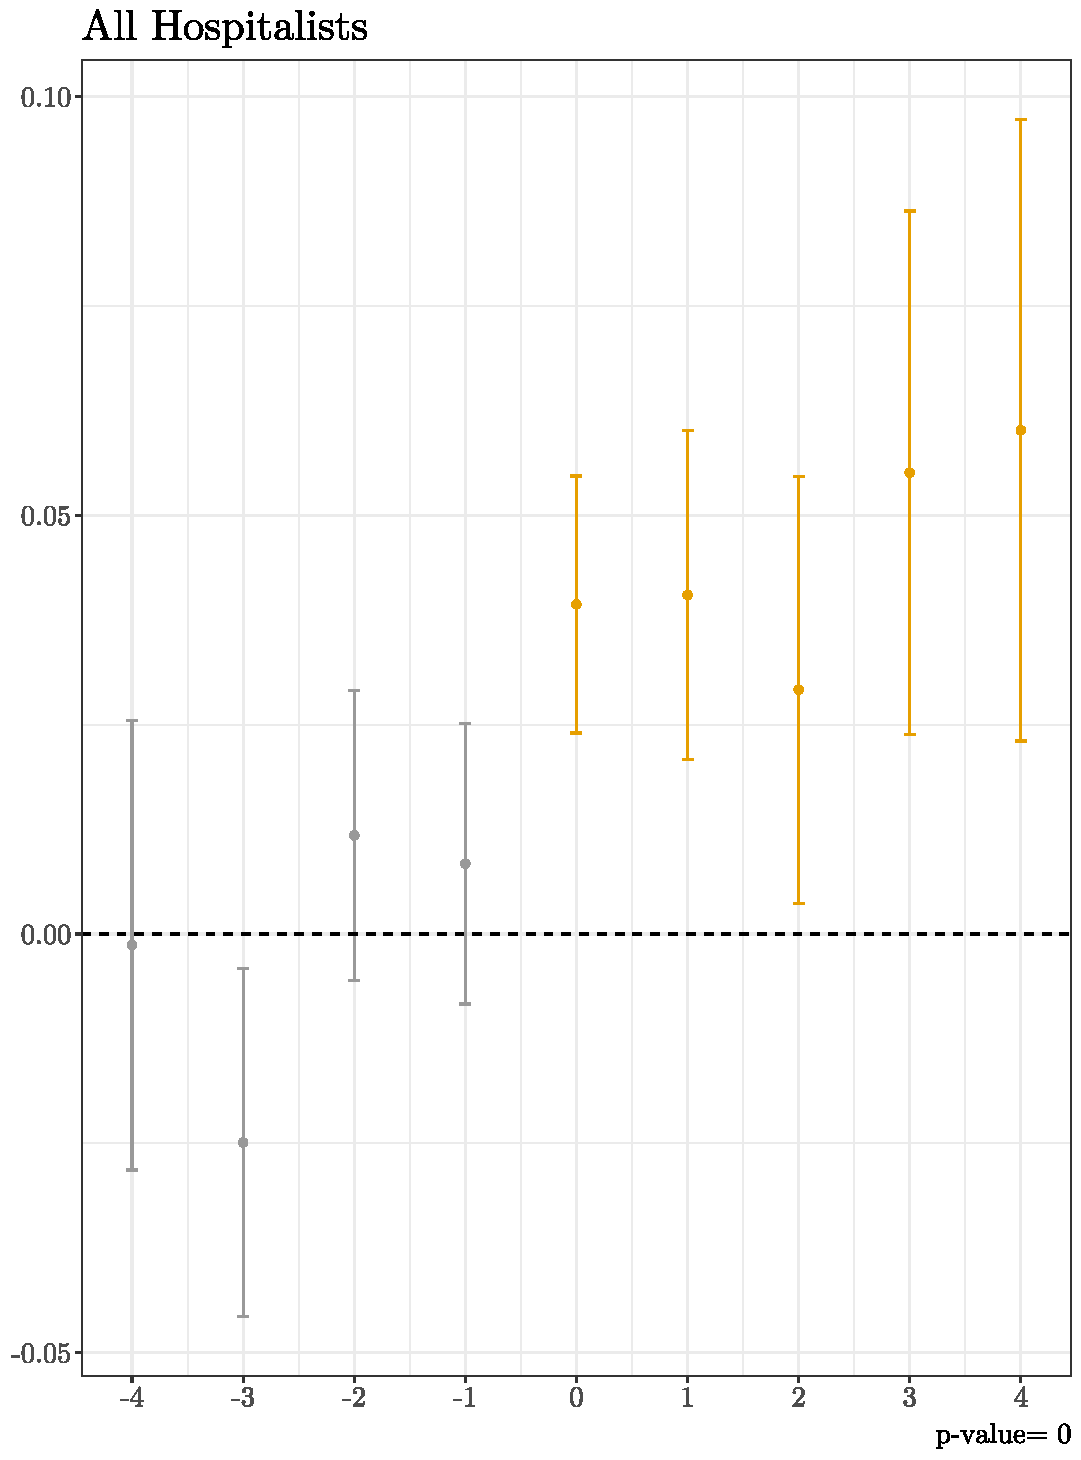
\includegraphics[scale=.35]{Objects/Presentation_zip_all.pdf}
\end{figure}
$\rightarrow$ Something happening in relative year -3, may be a pre-trend
\end{frame}

\begin{frame}{Results: Indicator for Changing Zip Codes}
\begin{figure}[ht]
    \centering
    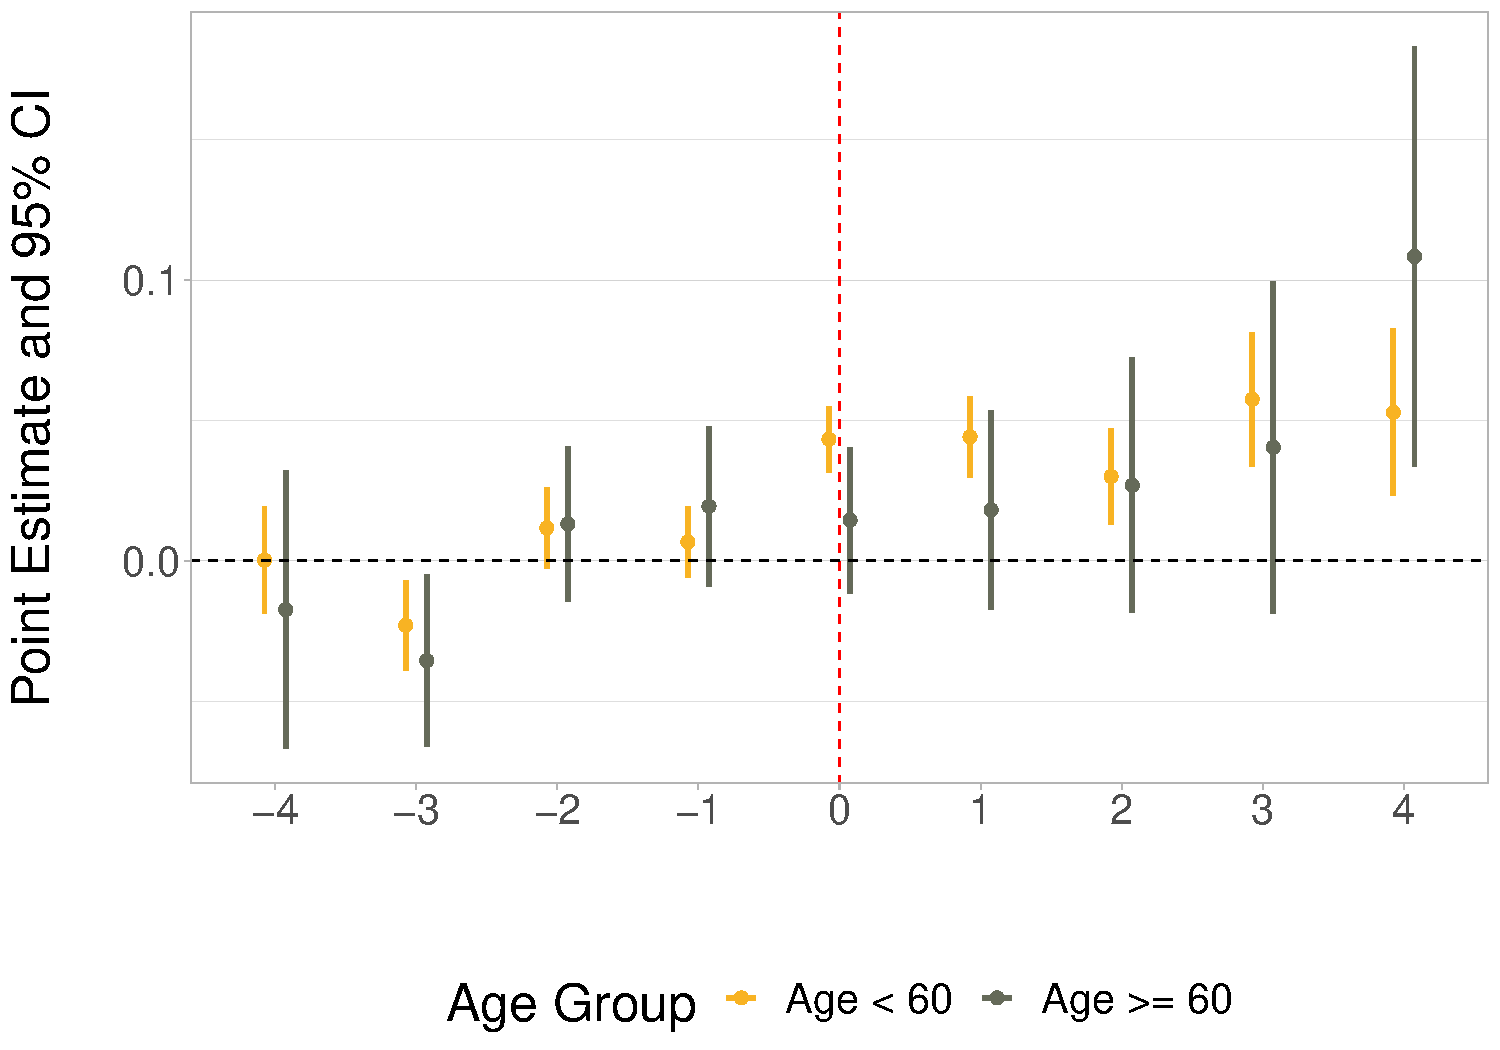
\includegraphics[scale=.35]{Objects/Presentation_zip_ages.pdf}
\end{figure}
$\rightarrow$ .043 ppt increase in likelihood of retiring for younger physicians (36\%)
$\rightarrow$ This effect is persistent
\end{frame}





\section{Productivity}





\begin{frame}{Productivity}
\centering
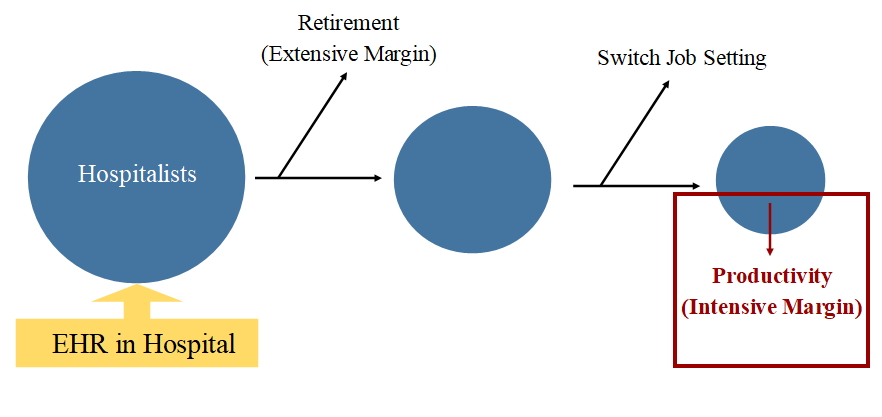
\includegraphics[scale=.45]{Objects/EHR_FlowChart_Productivity.PNG}
\end{frame}

\begin{frame}{Productivity Variables}
    \begin{enumerate}
        \item Patient count
        \vspace{6mm}
        \item Claims per patient
    \end{enumerate}
\end{frame}

\begin{frame}{Physician Incentives}
Past research on information technology $\rightarrow$ productivity typically increases \scriptsize (Bartel, Ichniowski and Shaw 2007, QJE)
                \vspace{3mm}
\begin{itemize}
                \normalsize 
    \item Sometimes depends on managerial style \scriptsize(Garicano and Heaton 2010, JLE)
\end{itemize}
                \vspace{6mm}
                \normalsize 
We can see how productivity is affected for physicians who don't change behavior as a result of EHRs
                \vspace{3mm}
\begin{itemize}
    \item Expected effect is ambiguous
                \vspace{3mm}
    \item Claim count per patient is a matter of physician incentives
\end{itemize}
\end{frame}

\begin{frame}{Results: Patient Count}
\begin{figure}[ht]
\centering
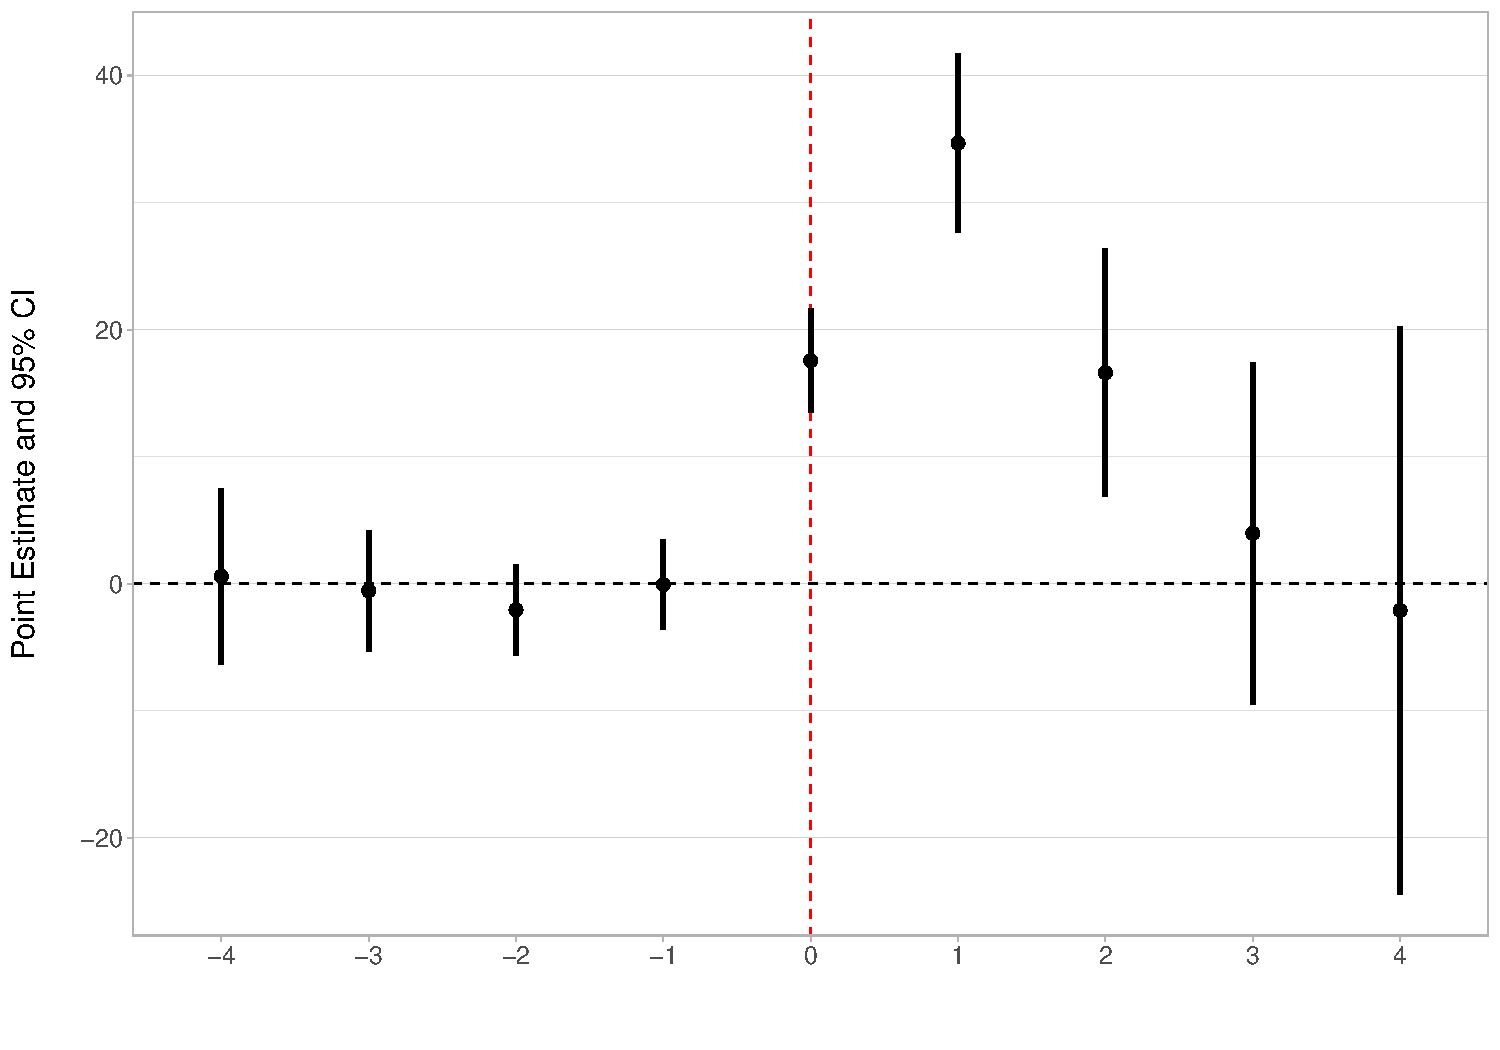
\includegraphics[scale=.35]{Objects/Presentation_patients_all.pdf}
\end{figure}
$\rightarrow$ 5-10\% increase relative to the mean\\
$\rightarrow$ Driven by demand? 
\end{frame}

\begin{frame}{Patient Count Broken Down by Group}
\centering
    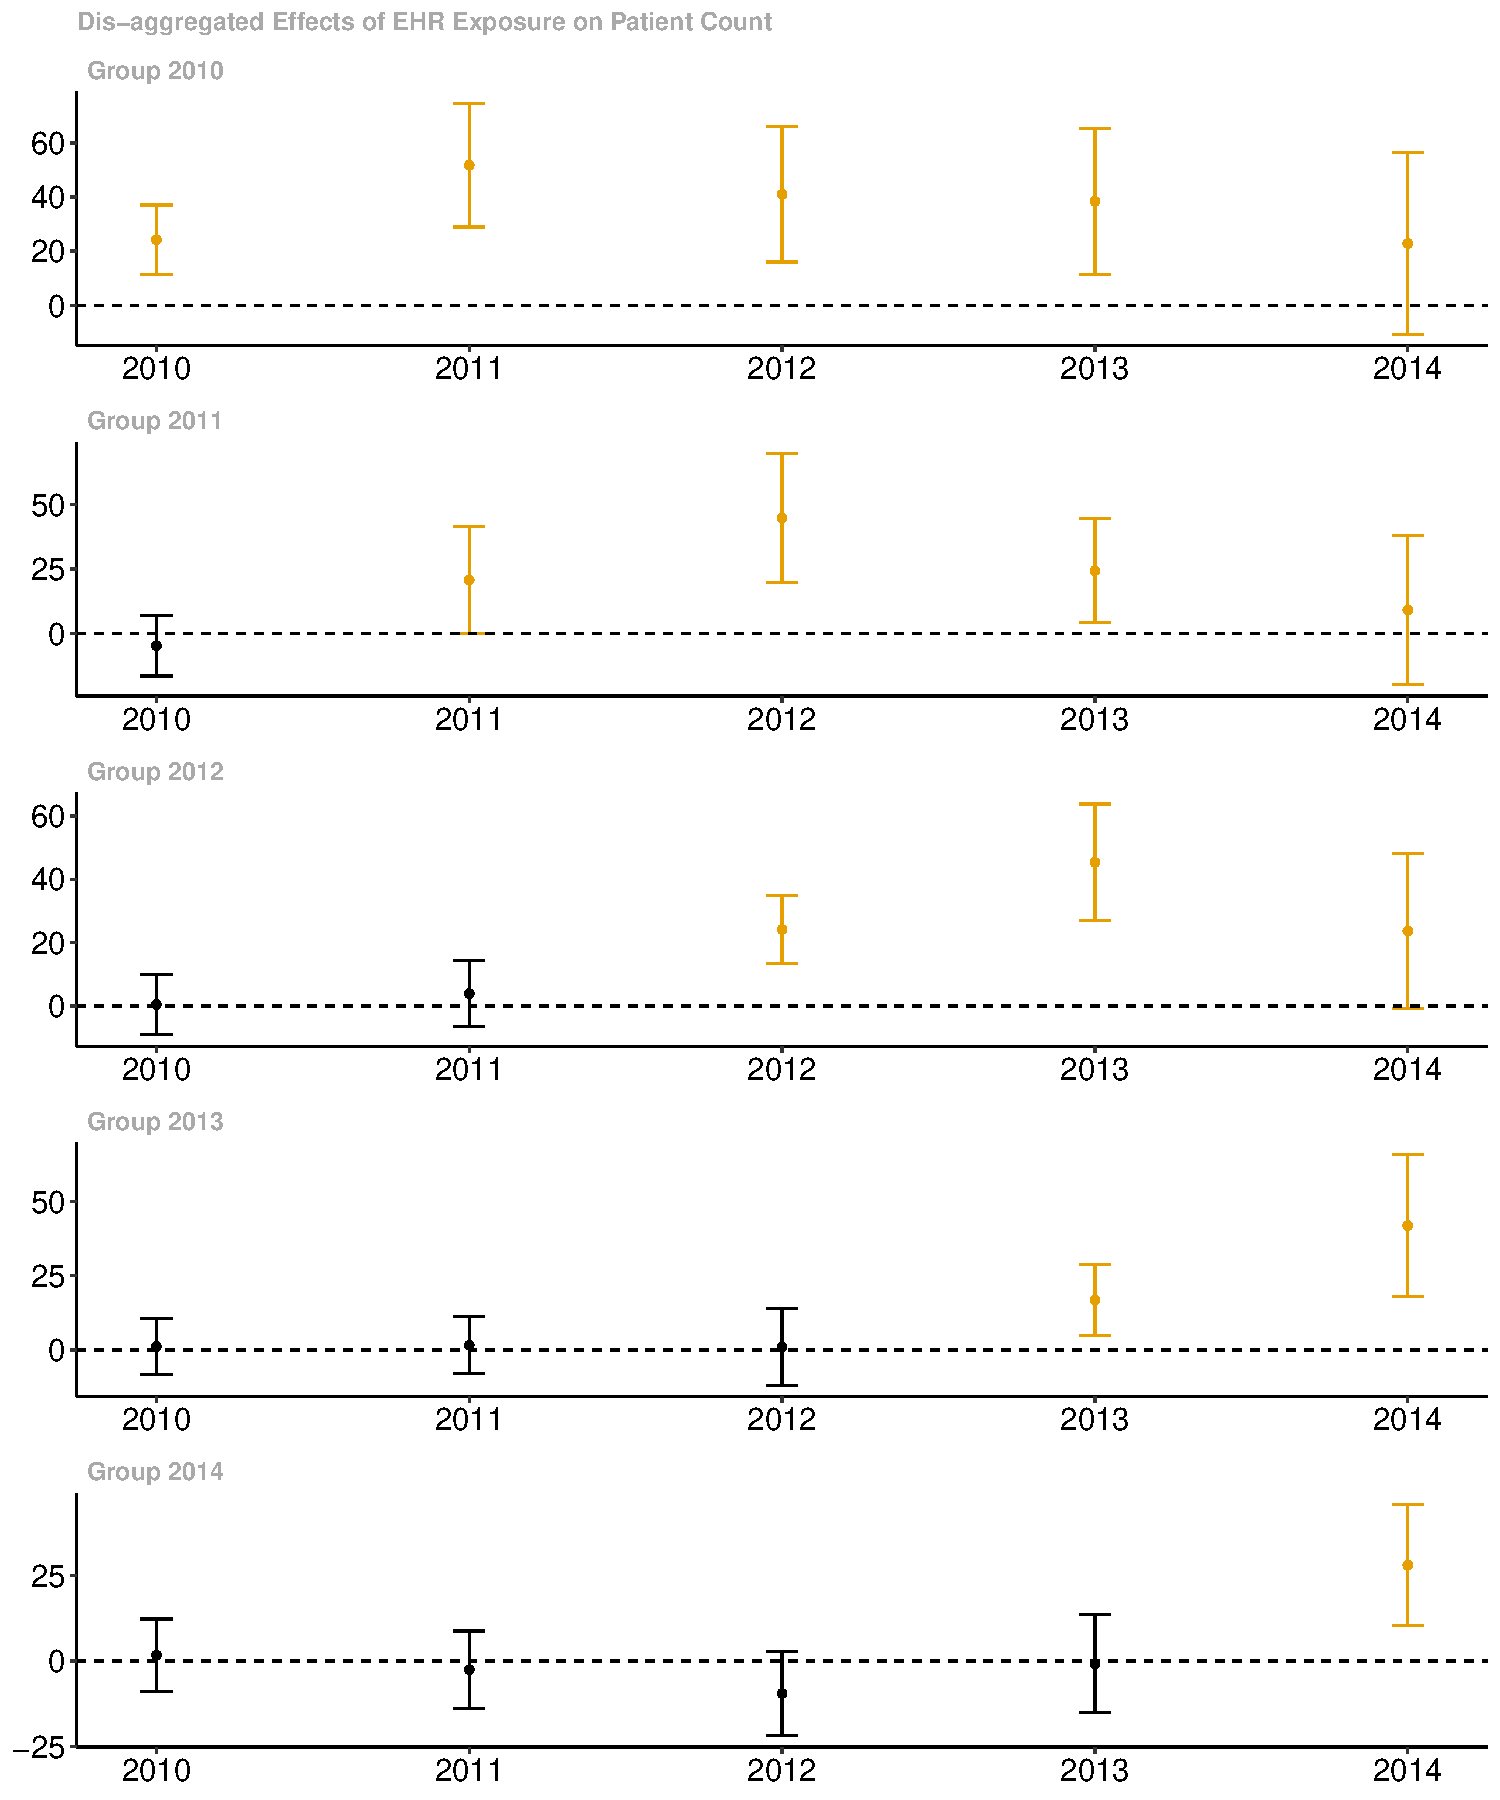
\includegraphics[scale=.25]{Objects/patient_group.pdf}
\end{frame}

\begin{frame}{Patient Count Broken Down by Age}
\begin{figure}[ht]
\centering
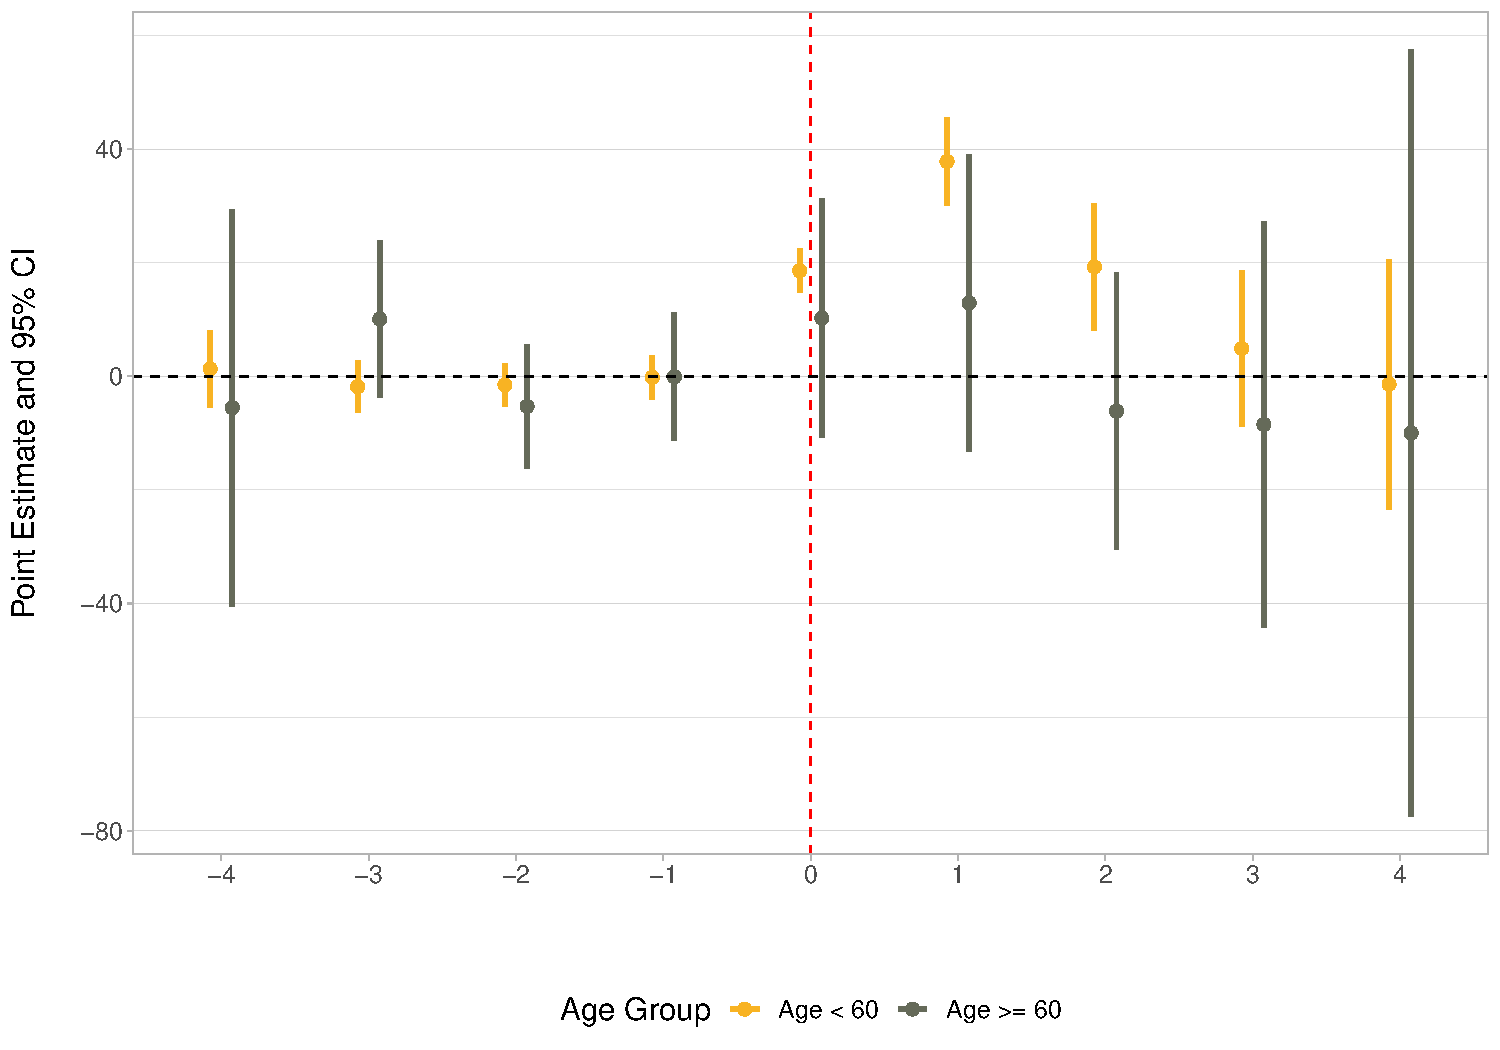
\includegraphics[scale=.4]{Objects/Presentation_patients_ages.pdf}
\end{figure}
$\rightarrow$ Don't see the same increase for older physicians
\end{frame}

\begin{frame}{Results: Claims per Patient}
\begin{figure}[ht]
\centering
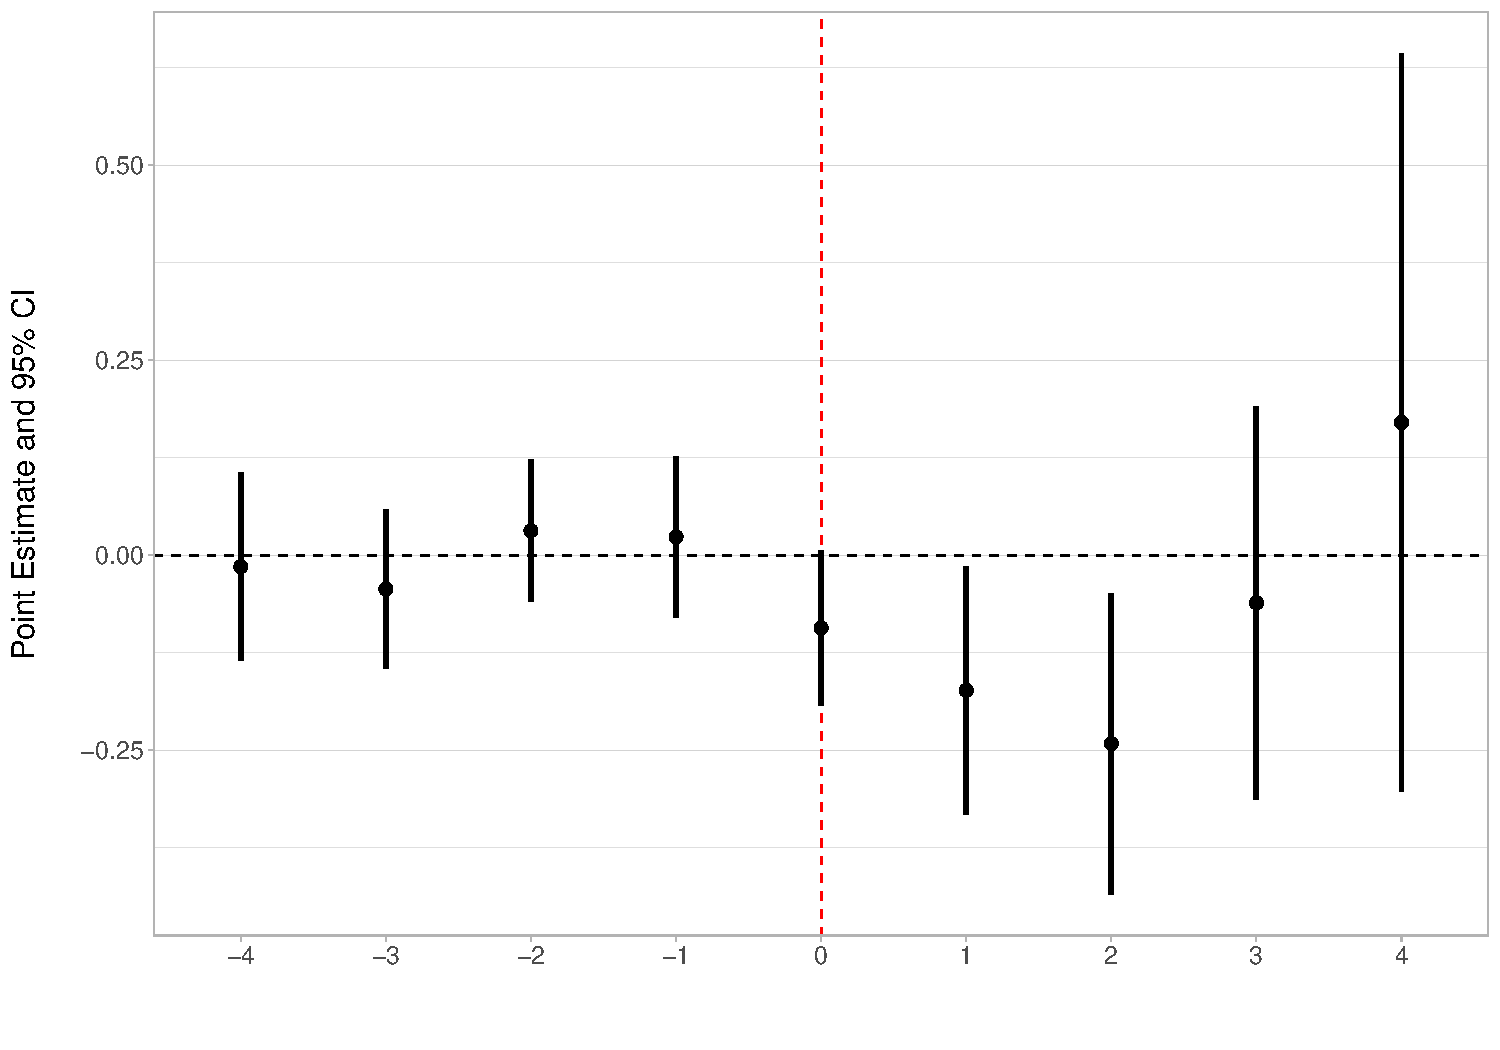
\includegraphics[scale=.35]{Objects/Presentation_claimperpatient_all.pdf}
\end{figure}
$\rightarrow$ Downward trend
\end{frame}



\section{Conclusion}


\begin{frame}{Summary}
\textcolor{red}{Downside}: evidence that physicians are changing their behavior because of this new technology\\
                \vspace{6mm}
\textcolor{teal}{Potential upside}: For physicians who endure through the implementation of the technology, number of patients goes up and claims per patient goes down

\end{frame}

\begin{frame}{Robustness Checks}
\begin{enumerate}
    \item Endogeneity of treatment
            \vspace{3mm}
    \item Data assistants
            \vspace{3mm}
    \item Limiting years and using never-treated as control
            \vspace{3mm}
    \item Anticipation
\end{enumerate}
\end{frame}


\begin{frame}[plain]{}
\centering
    Thank you! \\
    \vspace{5mm}
    Email: hkagele@emory.edu
\end{frame}



\end{document}